%%%%%%%%%%%%%%%%%%%%%%%%%%%%%%%%%%%%%%%%%
% Beamer Presentation
% LaTeX Template
% Version 1.0 (10/11/12)
%
% This template has been downloaded from:
% http://www.LaTeXTemplates.com
%
% License:
% CC BY-NC-SA 3.0 (http://creativecommons.org/licenses/by-nc-sa/3.0/)
%
%%%%%%%%%%%%%%%%%%%%%%%%%%%%%%%%%%%%%%%%%

%----------------------------------------------------------------------------------------
%	PACKAGES AND THEMES
%----------------------------------------------------------------------------------------

\documentclass{beamer}

\mode<presentation> {

% The Beamer class comes with a number of default slide themes
% which change the colors and layouts of slides. Below this is a list
% of all the themes, uncomment each in turn to see what they look like.

%\usetheme{default}
%\usetheme{AnnArbor}
%\usetheme{Antibes}
%\usetheme{Bergen}
%\usetheme{Berkeley}
%\usetheme{Berlin}
%\usetheme{Boadilla}
%\usetheme{CambridgeUS}
%\usetheme{Copenhagen}
%\usetheme{Darmstadt}
%\usetheme{Dresden}
%\usetheme{Frankfurt}
%\usetheme{Goettingen}
%\usetheme{Hannover}
%\usetheme{Ilmenau}
%\usetheme{JuanLesPins}
%\usetheme{Luebeck}
\usetheme{Madrid}
%\usetheme{Malmoe}
%\usetheme{Marburg}
%\usetheme{Montpellier}
%\usetheme{PaloAlto}
%\usetheme{Pittsburgh}
%\usetheme{Rochester}
%\usetheme{Singapore}
%\usetheme{Szeged}
%\usetheme{Warsaw}

% As well as themes, the Beamer class has a number of color themes
% for any slide theme. Uncomment each of these in turn to see how it
% changes the colors of your current slide theme.

%\usecolortheme{albatross}
%\usecolortheme{beaver}
%\usecolortheme{beetle}
%\usecolortheme{crane}
%\usecolortheme{dolphin}
%\usecolortheme{dove}
%\usecolortheme{fly}
%\usecolortheme{lily}
%\usecolortheme{orchid}
%\usecolortheme{rose}
%\usecolortheme{seagull}
%\usecolortheme{seahorse}
%\usecolortheme{whale}
%\usecolortheme{wolverine}

%\setbeamertemplate{footline} % To remove the footer line in all slides uncomment this line
%\setbeamertemplate{footline}[page number] % To replace the footer line in all slides with a simple slide count uncomment this line

\setbeamertemplate{navigation symbols}{} % To remove the navigation symbols from the bottom of all slides uncomment this line
}

\usepackage{graphicx} % Allows including images
%\usepackage{booktabs} % Allows the use of \toprule, \midrule and
                      % \bottomrule in tables
\usepackage{tikz}
\usepackage{tikz-cd}
\usepackage{varwidth}
\usepackage{amsmath}
\usepackage[author-year]{amsrefs}
\usepackage{../ReAdTeX/readtex-core}
% \usepackage{../ReAdTeX/readtex-dangerous}
% \usepackage{../ReAdTeX/readtex-abstract-algebra}
\usepackage{ytableau}
%%%%%%%%%%%%%%%%%%%%%%%%%%%%%%%%%%%%%%%%%%%%%%%%%%%%%%%%%%%%%%%%%%% 
%%  MACRO DEFINITIONS:  Co-authors -- PLEASE use these! 
%%%%%%%%%%%%%%%%%%%%%%%%%%%%%%%%%%%%%%%%%%%%%%%%%%%%%%%%%%%%%%%%%%%
\definecolor{coralred}{rgb}{1.0, 0.25, 0.25}
\definecolor{lightblue}{rgb}{.3,.65,1.0} %
\DeclareMathOperator{\Gr}{Gr}
\newcommand{\cupprod}{\cup}
\newcommand{\sym}{\Lambda}
\newcommand{\lowers}{\mathcal{L}}
\newcommand{\mynone}{\ }
\newcommand{\G}{\mathfrak{G}}
\renewcommand{\S}{\mathfrak{S}}
\DeclareMathOperator{\SSYT}{SSYT}
\renewcommand{\Span}{\operatorname{sp}}

%%%%%%%%%%%%%%%%%%%%%%%%%%%%%%%%%%%%%%%%%%%%%%%%%%%%%%%%%%%%%%%%%%%% 


%----------------------------------------------------------------------------------------
%	TITLE PAGE
%----------------------------------------------------------------------------------------

\title[Symmetric Functions]{A Window into Symmetric Function Theory} % The short title appears at the bottom of every slide, the full title is only on the title page

\author[George H. Seelinger]{George H. Seelinger} % Your name
\institute[UVA] % Your institution as it will appear on the bottom of every slide, may be shorthand to save space
{
  \medskip
\textit{ghs9ae@virginia.edu}\\ % Your email address
\medskip
UVA Math Club\\Lightning Round % Your institution for the title page
}
\date{2 March 2021} % Date, can be changed to a custom date
\begin{document}
\begin{frame}
 \titlepage 
\end{frame}
\begin{frame}{Symmetric Group}
  \begin{itemize}
  \item Permutations \(\sigma \from \{1,2,\ldots,n\} \to \{1,2,\ldots,n\}\):\pause \[
\left(
  \begin{matrix}
    1 & 2 & 3 & 4\\
    2 & 3 & 1 & 4 
  \end{matrix}
\right) = 
      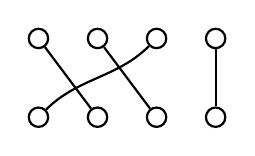
\begin{tikzpicture}[scale = 0.5,thick, baseline={(0,-1ex/2)}] 
        \tikzstyle{vertex} = [shape = circle, minimum size = 7pt, inner sep = 1pt] 
        \node[vertex] (G--4) at (4.5, -1) [shape = circle, draw] {}; 
        \node[vertex] (G-4) at (4.5, 1) [shape = circle, draw] {}; 
        \node[vertex] (G--3) at (3.0, -1) [shape = circle, draw] {}; 
        \node[vertex] (G-2) at (1.5, 1) [shape = circle, draw] {}; 
        \node[vertex] (G--2) at (1.5, -1) [shape = circle, draw] {}; 
        \node[vertex] (G-1) at (0.0, 1) [shape = circle, draw] {}; 
        \node[vertex] (G--1) at (0.0, -1) [shape = circle, draw] {}; 
        \node[vertex] (G-3) at (3.0, 1) [shape = circle, draw] {}; 
        \draw[] (G-4) .. controls +(0, -1) and +(0, 1) .. (G--4); 
        \draw[] (G-2) .. controls +(0.75, -1) and +(-0.75, 1) .. (G--3); 
        \draw[] (G-1) .. controls +(0.75, -1) and +(-0.75, 1) .. (G--2); 
        \draw[] (G-3) .. controls +(-1, -1) and +(1, 1) .. (G--1); 
      \end{tikzpicture}
    \] \pause
  \item Stacking = composition \pause \[
      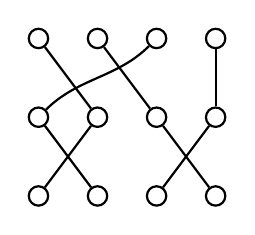
\begin{tikzpicture}[scale = 0.5,thick, baseline={(0,-3ex)}] 
        \tikzstyle{vertex} = [shape = circle, minimum size = 7pt, inner sep = 1pt] 
        \node[vertex] (G--4) at (4.5, -1) [shape = circle, draw] {}; 
        \node[vertex] (G-4) at (4.5, 1) [shape = circle, draw] {}; 
        \node[vertex] (G--3) at (3.0, -1) [shape = circle, draw] {}; 
        \node[vertex] (G-2) at (1.5, 1) [shape = circle, draw] {}; 
        \node[vertex] (G--2) at (1.5, -1) [shape = circle, draw] {}; 
        \node[vertex] (G-1) at (0.0, 1) [shape = circle, draw] {}; 
        \node[vertex] (G--1) at (0.0, -1) [shape = circle, draw] {}; 
        \node[vertex] (G-3) at (3.0, 1) [shape = circle, draw] {}; 
        \draw[] (G-4) .. controls +(0, -1) and +(0, 1) .. (G--4); 
        \draw[] (G-2) .. controls +(0.75, -1) and +(-0.75, 1) .. (G--3); 
        \draw[] (G-1) .. controls +(0.75, -1) and +(-0.75, 1) .. (G--2); 
        \draw[] (G-3) .. controls +(-1, -1) and +(1, 1) .. (G--1); 
        \node[vertex] (H--4) at (4.5, -3) [shape = circle, draw] {}; 
        \node[vertex] (H--3) at (3.0, -3) [shape = circle, draw] {}; 
        \node[vertex] (H--2) at (1.5, -3) [shape = circle, draw] {}; 
        \node[vertex] (H--1) at (0.0, -3) [shape = circle, draw] {}; 
        \draw[] (G--3) .. controls +(0.75, -1) and +(-0.75, 1) .. (H--4); 
        \draw[] (G--4) .. controls +(-0.75, -1) and +(0.75, 1) .. (H--3); 
        \draw[] (G--1) .. controls +(0.75, -1) and +(-0.75, 1) .. (H--2); 
        \draw[] (G--2) .. controls +(-0.75, -1) and +(0.75, 1) .. (H--1); 
      \end{tikzpicture}
      =
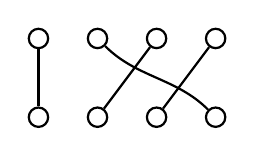
\begin{tikzpicture}[scale = 0.5,thick, baseline={(0,0)}] 
\tikzstyle{vertex} = [shape = circle, minimum size = 7pt, inner sep = 1pt] 
\node[vertex] (G--4) at (4.5, -1) [shape = circle, draw] {}; 
\node[vertex] (G-2) at (1.5, 1) [shape = circle, draw] {}; 
\node[vertex] (G--3) at (3.0, -1) [shape = circle, draw] {}; 
\node[vertex] (G-4) at (4.5, 1) [shape = circle, draw] {}; 
\node[vertex] (G--2) at (1.5, -1) [shape = circle, draw] {}; 
\node[vertex] (G-3) at (3.0, 1) [shape = circle, draw] {}; 
\node[vertex] (G--1) at (0.0, -1) [shape = circle, draw] {}; 
\node[vertex] (G-1) at (0.0, 1) [shape = circle, draw] {}; 
\draw[] (G-2) .. controls +(1, -1) and +(-1, 1) .. (G--4); 
\draw[] (G-4) .. controls +(-0.75, -1) and +(0.75, 1) .. (G--3); 
\draw[] (G-3) .. controls +(-0.75, -1) and +(0.75, 1) .. (G--2); 
\draw[] (G-1) .. controls +(0, -1) and +(0, 1) .. (G--1); 
\end{tikzpicture}
    \] \pause
  \item \(S_n\) is a ``group''
  \end{itemize}
\end{frame}
\begin{frame}{Polynomials}
  \begin{itemize}
  \item \(f \in \Q[x_1,\ldots,x_n]\) multivariate polynomial \pause
    \[
      \left(
        \begin{matrix}
          1 & 2 & 3\\
          3 & 2 & 1
        \end{matrix}
      \right) (5x_1^2+5x_2^2+8x_3^2) = 8x_1^2+5x_2^2+5x_3^2
    \]\pause
  \item \(\sigma \in S_n\) acts as \(\sigma.f(x_1,x_2,\ldots,x_n) =
    f(x_{\sigma(1)}, x_{\sigma(2)},\ldots,x_{\sigma(n)})\)
  \end{itemize}
\end{frame}
\begin{frame}{Symmetric Polynomials}
  \begin{itemize}
    \item Polynomials \(f \in \Q[x_1,\ldots,x_n]\) satisfying \(\sigma.f
    = f\)? \pause
  \item Symmetric polynomials (\(n=3\))
    \begin{align*}
      e_1 = x_1 + x_2 + x_3 = & h_1  \\
      e_2 = x_1 x_2 + x_1 x_3 + x_2 x_3 \quad & h_2 = x_1^2 + x_1 x_2 + x_1
                                          x_3 + x_2^2 +  x_2 x_3 +x_3^2  \\
      e_3 = x_1 x_2 x_3 \quad & h_3 = x_1^3 + x_1^2 x_2 + x_1^2 x_3 + x_1
                          x_2^2 + \cdots
    \end{align*} \pause
  \item \(\{f \in \Q[x_1,\ldots,x_n] \st \sigma.f = f \, \forall \sigma
    \in S_n\}\) forms a vector space, \(\sym_\Q\).
\end{itemize}
\end{frame}
\begin{frame}{Combinatorics of Symmetric Polynomials}
  \begin{block}{Generators}
    \[
      e_r =
      \sum_{i_1 < i_2 < \cdots < i_r} x_{i_1} x_{i_2} \cdots x_{i_r}
      \text { or }
      h_r = 
      \sum_{i_1 \leq i_2 \leq \cdots \leq i_r} x_{i_1} x_{i_2} \cdots x_{i_r}
    \]\pause 
  \end{block}
    Symmetric functions are polynomials in the \(e_1,e_2,\ldots\), or
    in the \(h_1,h_2,\ldots\) \[
     3 h_2 h_1^2 - h_2^2 + 6 h_3 h_1 = 3 h_{(211)} - h_{(22)} + 6 h_{(31)}
    \]
    \pause
    Basis of \(\sym_\Q\)?
\end{frame}
\begin{frame}{Partitions}
  \begin{definition}
    \(n \in \Z_{>0}\), a \emph{partition of \(n\)} is
    \(\lambda = (\lambda_1 \geq
    \lambda_2 \geq \cdots \geq \lambda_\ell > 0)\) such that
    \(\lambda_1+\lambda_2 + \cdots + \lambda_\ell = n \).
  \end{definition}\pause
  \ytableausetup{boxsize=0.5em, aligntableaux=center}
  \begin{align*}
    5 \to &\ \ydiagram{5} & 
    2+2+1 \to&\ \ydiagram{2,2,1}\\
    4+1 \to &\ \ydiagram{4,1}&
    2+1+1+1 \to&\ \ydiagram{2,1,1,1} \\
    3+2 \to &\ \ydiagram{3,2}&
    1+1+1+1+1 \to&\ \ydiagram{1,1,1,1,1}\\
    3+1+1 \to &\ \ydiagram{3,1,1}
  \end{align*}
\end{frame}
\begin{frame}{Partitions}
  Partitions by themselves are interesting!\pause
  \begin{enumerate}
  \item How many partitions of \(n\)? No known closed-form formula!\pause
  \item Many interesting connections to number theory (Ramanujan).\pause
  \item Generating function for \(p(n) =\) number of partitions of
    \(n\) is inverse of Euler \(\phi\) function.
  \end{enumerate}
\end{frame}
\begin{frame}{Tableaux}
  \begin{definition}
    Filling of partition diagram of \(\lambda\) with numbers such that\pause
    \begin{enumerate}
    \item strictly increasing down columns\pause
    \item weakly increasing along rows\pause
    \end{enumerate}
    Collection is called \(\SSYT(\lambda)\). \pause
  \end{definition}
  For \(\lambda = (2,1)\),
  \ytableausetup{aligntableaux=bottom,boxsize=1em}
\[
  \ytableaushort{11,2},\  \ytableaushort{11,3},\ \ytableaushort{22,3},\
    \ytableaushort{12,2},\ \ytableaushort{13,3},\ \ytableaushort{23,3},\
    \ytableaushort{13,2},\ \ytableaushort{12,3}
\]
\end{frame}
\begin{frame}{Schur functions}
  Associate a polynomial to \(\SSYT(\lambda)\).\pause
 \[
  \quad \quad \quad \quad \quad \quad \quad \quad \ytableaushort{11,2},\  \ytableaushort{11,3},\ \ytableaushort{22,3},\
    \ytableaushort{12,2},\ \ytableaushort{13,3},\ \ytableaushort{23,3},\
    \ytableaushort{13,2},\ \ytableaushort{12,3}
  \]\pause
  \[
    s_{(21)}(x_1,x_2,x_3) = x_1^2x_2+x_1^2x_3+x_2^2x_3+x_1x_2^2+x_1x_3^2+x_2x_3^2+2x_1x_2x_3
  \]\pause
  \begin{definition}
    For \(\lambda\) a partition \[
      s_\lambda = \sum_{T \in \SSYT} x^T \text{ for }x^T = \prod_{i
        \in T} x_i
    \]
  \end{definition}
  \pause
  \begin{itemize}
  \item \(s_\lambda\) is a symmetric function\pause
  \item Schur functions form a basis for \(\sym_\Q\) 
  \end{itemize}
\end{frame}
\begin{frame}{Why?}
  \begin{block}{Harmonic polynomials}
   \(M =\) polynomials killed by all symmetric differential
   operators.
  \end{block}\pause
  Explicitly, for
   \[
     \Delta = \det \left|
       \begin{matrix}
         x_1^2 & x_1 & 1\\
         x_2^2 & x_2 & 1\\
         x_3^2 & x_3 & 1
       \end{matrix}
     \right| = x_1^2(x_2-x_3) - x_2^2 (x_1 - x_3) + x_3^2(x_1-x_2)
   \]\pause
   \(M\) is the vector space given by\pause
   \begin{align*}
       M  = & \Span\left\{
\left(           \partial_{x_1}^a
           \partial_{x_2}^b  \partial_{x_3}^c
\right)         \Delta \st a,b,c \geq 0\right\} \\
        = & \Span\{\Delta, 2x_1(x_2-x_3)-x_2^2+x_3^2,
            2x_2(x_3-x_1)-x_3^2+x_1^2, \\
       & \phantom{\Span\{\}}x_3-x_1, x_2-x_3,1\}
   \end{align*}
\end{frame}
\begin{frame}{Harmonic polynomials}
  \begin{enumerate}
  \item \(S_3\) action on \(M\) fixes vector subspaces!
  \[
\Span\{\Delta, 2x_1(x_2-x_3)-x_2^2+x_3^2,
            2x_2(x_3-x_1)-x_3^2+x_1^2, 
       x_3-x_1, x_2-x_3,1\}
  \]\pause 
\item Break \(M\) up into smallest \(S_n\) fixed subspaces \pause
  \ytableausetup{boxsize=0.75em,aligntableaux=top}
  \[
    \hspace{-2.9em}
    \scalebox{0.95}{\(
      \underbrace{\Span\{\Delta\}}_{\ydiagram{1,1,1}} {\oplus} \underbrace{\Span\{2x_1(x_2{-}x_3){-}x_2^2{+}x_3^2,
        2x_2(x_3{-}x_1){-}x_3^2{+}x_1^2\}}_{\ydiagram{2,1}} {\oplus}
      \underbrace{\Span\{x_3{-}x_1, x_2{-}x_3\}}_{\ydiagram{2,1}} {\oplus} \underbrace{\Span\{1\}}_{\ydiagram{3}}\)}
  \]\pause
  \item How many times does an \(S_n\) fixed subspace occur? \pause
    Frobenius: \pause
    \ytableausetup{boxsize=0.5em}
    \[
      e_1^3 = (x_1+x_2+x_3)^3 = s_{\ydiagram{1,1,1}} + s_{\ydiagram{2,1}} +
      s_{\ydiagram{2,1}} + s_{\ydiagram{3}}
    \]
  \end{enumerate}
  \pause
  Schur basis expansion counts multiplicity of irreducible \(S_n\)
  fixed subspaces!
\end{frame}
\begin{frame}{Schur positivity}
  \begin{block}{Upshot}
    \begin{enumerate}
      \pause
    \item Schur functions \(\correspondsto\) \(S_n\)-invariant
      subspaces.\pause
    \item Via Frobenius characteristic map, questions about
      \(S_n\)-action on vector spaces get translated to questions
      about Schur expansion coefficients in symmetric functions.
    \end{enumerate}
  \end{block}
\end{frame}
\begin{frame}{Schur positivity}
    \begin{block}{Interesting algebraic combinatorics questions}
    \begin{enumerate}
      \pause
    \item Is a symmetric function Schur positive?
      \pause
    \item What do the Schur expansion coefficients count?
    \end{enumerate}
  \end{block}
\end{frame}
\begin{frame}{Getting more information}
  \pause
  Break \(M\) up into smallest \(S_n\) fixed subspaces 
  \ytableausetup{boxsize=0.75em,aligntableaux=top}
  \[
    \hspace{-0.75em}
    \scalebox{0.95}{\(
      \underbrace{\Span\{\Delta\}}_{\ydiagram{1,1,1}} {\oplus} \underbrace{\Span\{2x_1(x_2{-}x_3){-}x_2^2{+}x_3^2,
        2x_2(x_3{-}x_1){-}x_3^2{+}x_1^2\}}_{\substack{\ydiagram{2,1}\\\deg
        = 2}} {\oplus}
      \underbrace{\Span\{x_3{-}x_1, x_2{-}x_3\}}_{\substack{\ydiagram{2,1}\\\deg=1}} {\oplus} \underbrace{\Span\{1\}}_{\ydiagram{3}}\)}
  \]
  \pause
  Solution: minimal \(S_n\)-fixed subspace of degree \(d\) \(\mapsto q^d
  s_\lambda\) (graded Frobenius)\[
    ?? = q^3 s_{\ydiagram{1,1,1}} + q^2 s_{\ydiagram{2,1}} + q
    s_{\ydiagram{2,1}} + s_{\ydiagram{3}}
  \]\pause
\end{frame}
\begin{frame}{An example of bi-degree}
  Capturing even more information...\pause
  \begin{itemize}
  \item \(\Q[x_1,\ldots,x_n,y_1,\ldots,y_n]\) satisfying
    \(\sigma(x_i) = x_{\sigma(i)}\), \(\sigma(y_j) = y_{\sigma(j)}\).\pause
  \item Garsia-Haiman: \(M_\mu = \) span of partial derivatives of
    \(\Delta_\mu\) \pause \[
      \Delta_{\ydiagram{2,1}} = \det \left|
        \begin{matrix}
          1 & y_1 & x_1 \\
          1 & y_2 & x_2 \\
          1 & y_3 & x_3
        \end{matrix}
      \right| = x_3 y_2 - y_3 x_2 - y_1 x_3 + y_1 x_2 + y_3 x_1 - y_2 x_1
    \]
    \pause
  \[
    \hspace{-1em}
      M_{2,1} = \underbrace{\Span\{\Delta_{2,1}\}}_{\deg = (1,1)}
      \oplus \underbrace{\Span\{y_3-y_1, y_1 - y_2\}}_{\deg = (0,1)}
      \oplus \underbrace{\Span\{x_3-x_1, x_1 - x_2\}}_{\deg = (1,0)}
      \oplus \underbrace{\Span \{1\}}_{\deg = (0,0)}
    \]
    \pause
    Minimal \(S_n\)-invariant subspace with bidegree \((a,b) \mapsto
    q^at^b s_\lambda\) \pause \[
      \tilde{H}_\mu = qt s_{\ydiagram{1,1,1}} + t
      s_{\ydiagram{2,1}} + q s_{\ydiagram{2,1}} + s_{\ydiagram{3}}
    \]
  \end{itemize}
\end{frame}
\begin{frame}{Diagonal harmonics}
  \begin{itemize}
  \item Define \(\nabla\) by \(\nabla \tilde{H}_\mu = B_\mu(q,t) \tilde{H}_\mu\) for
    eigenvalue \(B_\mu(q,t) \in \Q[q,t]\). \[
      \nabla \tilde{H}_{2,1} = qt \tilde{H}_{2,1}
    \]\pause
  \item \(\hat{M} = \left\{ f \in \Q[x_1,\ldots,x_n,y_1,\ldots,y_n] \st
    \sum_{1 \leq j \leq n} \partial_{x_j}^a \partial_{y_j}^b f(x,y) =
    0 \right\}\).\pause
\item \(\hat{M} \to  \nabla e_n\)
  \ytableausetup{boxsize=0.5em}
  \[
    \nabla e_3 = (q^3+q^2t+qt^2+t^3+qt)s_{\ydiagram{1, 1, 1}} + (q^2+qt+t^2+q+t)s_{\ydiagram{2, 1}} + s_{\ydiagram{3}}
  \]\pause
    \end{itemize}
    \begin{block}{Open question}
      \pause
      What is the Schur expansion of \(\nabla e_n\)?
      \pause
    \end{block}
    Recover earlier story by taking \(t=0\) and \(y_i = 1\) for all \(y_i\)'s.
\end{frame}
\end{document}
%%% Local Variables:
%%% mode: latex
%%% TeX-master: t
%%% End:
